\documentclass{article}
%%%%%%%%%%%%%
% Loads packages
%%%%%%%%%%%%%
\usepackage[table]{xcolor}
\usepackage[utf8]{inputenc}
\usepackage[colorlinks=true,linkcolor=blue]{hyperref}
\usepackage{geometry} %package needed to set margins
\usepackage{fancyhdr}
\usepackage{graphicx}
\usepackage{amsmath}
\usepackage{amsthm}
\usepackage{mdframed}
\usepackage{tikz}
\usetikzlibrary{arrows.meta}
\usetikzlibrary{decorations.markings}
\usepackage{amsfonts}
\usepackage{wasysym}
\usepackage{listings}% http://ctan.org/pkg/listings
\lstset{
basicstyle=\ttfamily,
mathescape
}
\pagestyle{fancy}
\fancyhf{}
\chead{\textbf{Homework 8}}
\lhead{Math 213, Fall 2024}
\rhead{Due Sunday, 11/3 at 11:59pm}
%%%%%%%%%%%%%
% Sets margins
%%%%%%%%%%%%%
\newgeometry{left=1.5in,right=1in,top=1in,bottom=1in}
\setlength\headsep{3pt}
%%%%%%%%%%%%%
% Creates problem and solution environments
%%%%%%%%%%%%%
% Solution Environment
\newenvironment{solution}{\begin{proof}[Solution]}{\end{proof}}
% Problem Environment
\newenvironment{problem}[1]
{\begin{mdframed}[default]
\textbf{Problem #1:}
}
{\end{mdframed}
}
%%%%%%%%%%%
% Custom Commands
%%%%%%%%%%%
\newcommand{\gOne}{\cellcolor{green!50!white} 1}
\newcommand{\rZero}{\cellcolor{red!50!white} 0}
\begin{document}
\begin{problem}{\S 8.6 - 3}
How many solutions does the equation $x_1 + x_2 + x_3 = 13$ have where $x_1, x_2,$
and $x_3$ are nonnegative integers less than 6?

Solution:

To figure out this problem, we use inclusive-exclusive, Thus, $T=N_{total}-N(P)+N(P_iP_j)-N(P_iP_jP_k)$
For each $x$, since less than 6, the counter is $x\geq6$, then for every of them, we have ${13-6+3-1\choose 2}={9\choose 2}$, with three of them which is ${3\choose 1}$.

Then, find two that contradict, Which is ${3\choose 2}{13-6-6+3-1\choose 2}={3\choose 2}{3\choose 2}$.

And for all contradict, it is impossible, $since 13-6-6-6<0$
And total is ${13+3-1\choose 2}$\
So, Answer is: \[T={15\choose 2}-{3\choose 1}{9\choose 2}+{3\choose 2}{3\choose 2}=105-108+9=6\]
\end{problem}
\begin{problem}{\S 8.6 - 10}
In how many ways can eight distinct balls be distributed into three distinct urns
if each urn must contain at least one ball?

Solution, this is same as finding onto functions, so, using inclusive-exclusive.

$T=3^8 C(3,1)2^8+C(3,2)1^8=5796$
\end{problem}
\begin{problem}{\S 8.6 - 14}
What is the probability that none of 10 people receives the correct hat if a
hatcheck person hands their hats back randomly?

Solution:

This is a derangement problem, using the formula, $n!(1-\frac{1}{1!}+\frac{1}{2!}-\frac{1}{3!}+\cdots +(-1)^n\frac{1}{n!})$
since there are 10 elements, so, total derangement: $10!(1-\frac{1}{1!}+\frac{1}{2!}-\frac{1}{3!}+\cdots +(-1)^{10}\frac{1}{10!})$
And the probability should be \[P=1-\frac{1}{1!}+\frac{1}{2!}-\frac{1}{3!}+\cdots +(-1)^{10}\frac{1}{10!}\]
\end{problem}
\begin{problem}{\S 9.1 - 6(a-f)}
Determine whether the relation $R$ on the set of all real number is reflexive,
symmetric, antisymmetric, and/or transitive, where $(x,y) \in R$ if and only if
\begin{itemize}
\item[(a)] $x+y = 0$.
\item[(b)] $x = \pm y$.
\item[(c)] $x-y$ is a rational number.
\item[(d)] $x = 2y$.
\item[(e)] $xy \geq 0$.
\item[(f)] $xy = 0$.
\end{itemize}

Solution:
\begin{itemize}
\item[(a)] Since $1+1\neq0$, not reflexive. Since $x+y=y+x$, symmetric. Since $(1,(-1))=((-1),1)=0\in R$, so is not antisymmetric. Since $(1,(-1))\in R$, $((-1),1)\in R$, $(1,1)\notin R$, is not transitive.
\item[(b)] Since $x = \pm x$ (choosing the plus sign), the relation is reflexive. Since $x = \pm y$ if and only if $y =\pm x$,
the relation is symmetric. Since (1,-1) and (-1,1) are both in R, the relation is not antisymmetric. The
relation is transitive, essentially because the product of 1s and 1s is 1.
\item[(c)] Since $x-x=0$, and 0 is rational number, so it is reflexive. Since if $(x-y)$ is rational, $(y-x)=-(x-y)$ is also rational, it is symmetric. And since $1-(-1)$ and $(-1)-1$ are rational, and $1\neq -1$, it is not antisymmetric. And since as we assume $(x,y)$ and $(y,z)$ in R, when we do minus between $(x-y) and (y-z)$, we get $(x-z)$ is also in R, so it is transitive.
\item[(d)] Since $1\neq 1\times 2$, it is not reflexive. Since $(2,1)$ in R but $(1,2)$ not in R, it is not symmetric. Since suppose $x=2y$ in R, if $y=2x$ in R, only possible answer is x=y=0, so, it is antisymmetric. And since $(4,2)$ and $(2,1)$ in R, but $(4,1)$ not in R, so it is not transitive.
\item[(e)] Since $xx=x^2\geq 0$ by mathematics, it is reflexive. And since $xy=yx\geq 0$, $(x,y)$ and $(y,x)$ all in R, thus, it is symmetric. And since $(1,2)$ and $(2,1)$ in R, so it is not antisymmetric. And since $(1,0)$, $(0,-1)$ in R, but $(1,-1)$ not in R, so it is not transitive.
\item[(f)] Since $1\times 1 \neq 0$ not in R, so it is not reflexive. And since as $xy=yx$, so if $(x,y)$ in R, $(y,x)$ in R, so it is symmetric. And since $(1,0)$ and $(0,1)$ in R, thus, it is not antisymmetric. And since $(1,0)$ and $(0,2)$ in R, but $(1,2)$ not in R, so it is not transitive.
\end{itemize}

\end{problem}
\begin{problem}{\S 9.1 - 15}
Can a relation on a set be neither reflexive nor irreflexive?

Solution:

The definition of reflexive is if $(a,a) \in R$ for every element $a \in A$
and irreflexive is if $(a,a) \notin R$ for every element $a \in A$
So, in case of some $(a,a)\in R$, and some $(b,b)\notin R$, it is neither reflexive nor irreflexive.
like, there is a set $\{a,b,c\}$, and the relation is set $\{(a,a), (a,b), (b,c)\}$, since $(b,b)$ and $(c,c)$ not in R, it is not reflexive; and since $(a,a)$ in R, it is not irreflexive.

\end{problem}
\begin{problem}{\S 9.1 - 22}
Must an asymmetric relation also be antisymmetric? Must an antisymmetric relation
also be asymmetric?

The definition of a asymmetric relation is for all $x$ and $y$, $(x,y)$ in R but $(y,x)$ not in R, 

The definition of a antisymmetric relation is for every elements, if $(x,y)$ then $(y,x)$ then we can get $x=y$.

Assume $R$ is asymmetric. By definition, if $(x,y)\in R$, then $(y,x)\notin R$. Antisymmetry Condition: If,$(x,y)\in R$ and $(y,x)\in R$, then $x=y$. Given Asymmetry: The condition $(x,y)\in R$ and $(y,x)\in R$ never occurs unless $x=y$. Therefore: The antisymmetric condition is vacuously satisfied because the premise $(x,y)\in R$ and $(y,x)\in R$ cannot both be true unless $x=y$.
Conclusion: Asymmetric relations are always antisymmetric. Therefore, the proposition: "Must an asymmetric relation also be antisymmetric?" is true.

And for second proposition, since antisymmetric is both $(x,y)$ and $(y,x)$ in R can only be satisfy as $x=y$, so as asymmetric cannot satisfy every both $(x,y)$ and $(y,x)$ in R, it is false.
\end{problem}
\begin{problem}{\S 9.1 - 26}
Let $R$ be the relation $R = \{ (a,b) : a < b \}$ on the set of integers. Find
\begin{itemize}
\item[(a)] $R^{-1}$.
\item[(b)] $\overline{R}$.
\end{itemize}
Solution:

\begin{itemize}
    \item[(a)] $R^{-1}=\{(b,a):a<b\}$. Since it should be the reverse that is from B to A
    \item[(b)] $\overline{R}=\{(a,b):a\geq b\}$. Since it should be the complementary of R
    \end{itemize}
\end{problem}
\begin{problem}{\S 9.3 - 2(a,b)}
Represent each of these relations on $\{ 1, 2, 3, 4 \}$ with a matrix (with the
elements of this set listed in increasing order).
\begin{itemize}
\item[(a)] $\{ (1,2),~(1,3),~(1,4)~,(2,3),~(2,4),~(3,4) \}$
\item[(b)] $\{ (1,1),~(1,4),~(2,2),~(3,3),~(4,1) \}$
\end{itemize}

Solution:

\begin{itemize}
    \item[(a)] $\{ (1,2),~(1,3),~(1,4)~,(2,3),~(2,4),~(3,4) \}=\begin{bmatrix} 0&1&1&1 \\ 0&0&1&1 \\ 0&0&0&1 \\ 0&0&0&0 \end{bmatrix}$
    \item[(b)] $\{ (1,1),~(1,4),~(2,2),~(3,3),~(4,1) \}=\begin{bmatrix} 1&0&0&1 \\ 0&1&0&0 \\ 0&0&1&0 \\ 1&0&0&0 \end{bmatrix}$
    \end{itemize}
\end{problem}
\begin{problem}{\S 9.3 - 14(a-d)}
Let $R_1$ and $R_2$ be relations on a set $A$ represented by the matrices
\begin{align*}
M_{R_1} = \begin{bmatrix} 0 & 1 & 0 \\ 1 & 1 & 1 \\ 1 & 0 & 0 \end{bmatrix} \
qquad \textrm{and} \qquad
M_{R_2} = \begin{bmatrix} 0 & 1 & 0 \\ 0 & 1 & 1 \\ 1 & 1 & 1 \end{bmatrix}
\end{align*}
Find the matrices that represent
\begin{itemize}
\item[(a)] $R_1 \cup R_2$.
\item[(b)] $R_1 \cap R_2$.
\item[(c)] $R_2 \circ R_1$.
\item[(d)] $R_1 \circ R_1$.
\end{itemize}

Solution:

\begin{itemize}
    \item[(a)] $R_1 \cup R_2=\begin{bmatrix}0&1&0 \\1&1&1 \\ 1&1&1 \end{bmatrix}$.
    \item[(b)] $R_1 \cap R_2=\begin{bmatrix}0&1&0 \\0&1&1 \\ 1&0&0 \end{bmatrix}$.
    \item[(c)] $R_2 \circ R_1=\begin{bmatrix}0&1&1 \\1&1&1 \\ 0&1&0 \end{bmatrix}$.
    \item[(d)] $R_1 \circ R_1=\begin{bmatrix}1&1&1 \\1&1&1 \\ 0&1&0 \end{bmatrix}$.
    \end{itemize}
\end{problem}
\begin{problem}{\S 9.3 - 22}
Draw the directed graph that represents the relation \[ \{ (a,a),~(a,b),~(b,c),~(c,b),~(c,d),~(d,a),~(d,b) \}. \]

\begin{center}
    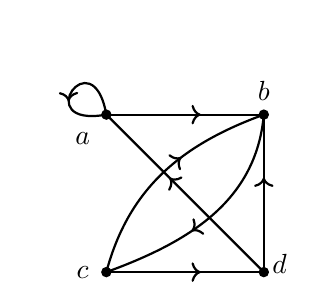
\begin{tikzpicture}
    \begin{scope}[thick,decoration={
    markings,
    mark=at position 0.6 with {\arrow{>}}}
    ]
    % draw vertices
    \node[circle, fill=black,scale = 0.4] at (0,0){};%c
    \node[circle, fill=black,scale = 0.4] at (2,0){};%d
    \node[circle, fill=black,scale = 0.4] at (0,2){};%a
    \node[circle, fill=black,scale = 0.4] at (2,2){};%b
    % draw directed edges
    \draw[postaction={decorate}] (0,0) to (2,0);%cd
    \draw[postaction={decorate}] (2,0) to (2,2);%db
    \draw[postaction={decorate}] (0,2) to (2,2);%ab
    \draw[postaction={decorate}] (2,0) to (0,2);%da
    \draw[postaction={decorate},out=75,in=200] (0,0) to (2,2);%bc
    \draw[postaction={decorate},out=-95,in=20] (2,2) to (0,0);%cb


    \draw[scale=2,postaction={decorate}] (0,1) to[out=100, in=190,loop] (0,1);%aa

    % labels vertices
    \node at (-0.3,0) {$c$};
    \node at (2.2,0.1) {$d$};
    \node at (-0.3,1.7) {$a$};
    \node at (2,2.3) {$b$};
    \end{scope}
    \end{tikzpicture}
    \end{center}

\end{problem}
\begin{problem}{\S 9.3 - 26}
List the ordered pairs in the relations represented by the directed graph
\begin{center}
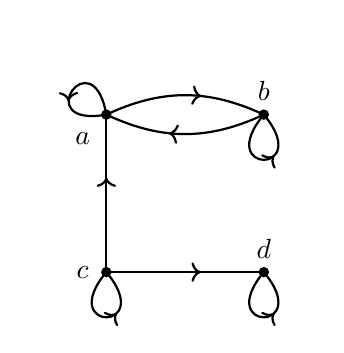
\begin{tikzpicture}
\begin{scope}[thick,decoration={
markings,
mark=at position 0.6 with {\arrow{>}}}
]
% draw vertices
\node[circle, fill=black,scale = 0.4] at (0,0){};
\node[circle, fill=black,scale = 0.4] at (2,0){};
\node[circle, fill=black,scale = 0.4] at (0,2){};
\node[circle, fill=black,scale = 0.4] at (2,2){};
% draw directed edges
\draw[postaction={decorate}] (0,0) to (2,0);
\draw[postaction={decorate}] (0,0) to (0,2);
\draw[postaction={decorate},out=25,in=155] (0,2) to (2,2);
\draw[postaction={decorate},out=205,in=-25] (2,2) to (0,2);
\draw[scale=2,postaction={decorate}] (0,0) to[out=-130,in=-50,loop] (0,0);
\draw[scale=2,postaction={decorate}] (0,1) to[out=100, in=190,loop] (0,1);
\draw[scale=2,postaction={decorate}] (1,0) to[out=-130,in=-50,loop] (1,0);
\draw[scale=2,postaction={decorate}] (1,1) to[out=-130,in=-50,loop] (1,1);
% labels vertices
\node at (-0.3,0) {$c$};
\node at (2,0.3) {$d$};
\node at (-0.3,1.7) {$a$};
\node at (2,2.3) {$b$};
\end{scope}
\end{tikzpicture}
\end{center}
Solution:

Ordered pairs:
\[(a,a),(a,b),(b,b),(b,a),(c,a),(c,c),(c,d),(d,d)\]
\end{problem}
\end{document}